\chapter{Unified Process (UP)}

\section{OOA e OOD}

\dfn{OOA/D}{
    \begin{itemize}
        \item \textbf{OOA} (Object Oriented Analysis): studio dei requisiti e delle specifiche del sistema;
        \item \textbf{OOD} (Object Oriented Design): progettazione del sistema.
    \end{itemize}

    Per studiare OOA/D si utilizza Unified Process, 
    un processo di sviluppo software orientato agli oggetti.
}

\nt{UP può essere applicato usando un 
approccio agile come Scrum o XP.}

\cor{UML}{
    UP utilizza UML come linguaggio di modellazione.
    UML è un linguaggio di modellazione grafico e testuale
    per la specifica, la costruzione e la documentazione
    di sistemi software orientati agli oggetti.

    \paragraph{IMPORTANTE:} UML non è nato per descrivere software, ma
    per descrivere concetti\footnote{Simile a ER, visto nel corso "Basi di dati".}.
}

\subsubsection{OOD è guidata dalle responsabilità (si vedano
i pattern GRASP):}

\begin{itemize}
    \item [$\Rightarrow$] Quali sono gli oggetti? Quali sono le classi?
    \item [$\Rightarrow$] Cosa deve conoscere un oggetto? Cosa deve saper fare?
    \item [$\Rightarrow$] Come collaborano gli oggetti?
\end{itemize}

\dfn{Pattern}{
    I pattern sono euristiche, best practice, che aiutano a codificare principi
    di soluzioni.
}


\subsubsection{ODD è correlata all'analisi dei requisiti:}

\begin{itemize}
    \item [$\Rightarrow$] \fancyglitter{Casi d'uso};
    \item [$\Rightarrow$] \fancyglitter{Storie utente}.
\end{itemize}
\pagebreak
\ex{Gioca una \newfancyglitter{partita a dadi}}{
\subsubsection{Definizione dei casi d'uso: storie scritte.}

Il \newfancyglitter{Giocatore} chiede
di \fancyglitter{lanciare} i \newfancyglitter{dadi}. Il Sistema presenta il
\fancyglitter{risultato}: se \fancyglitter{il valore totale} delle facce dei dadi
è sette, il giocatore ha vinto; altrimenti ha
perso.

\subsubsection{Definizione di un modello di dominio:
\newfancyglitter{i concetti o gli oggetti significativi}.}

\begin{center}
    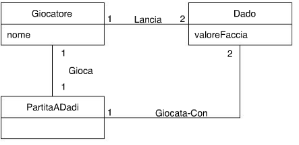
\includegraphics[scale=0.7]{images/Dadi.png}
\end{center}

\subsubsection{Assegnare responsabilità agli oggetti e 
disegnare diagrammi di interazione: \fancyglitter{responsabilità e collaborazioni}.}

\begin{center}
    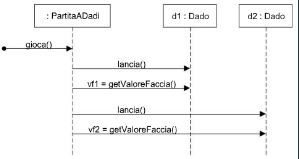
\includegraphics[scale = 0.7]{images/Dadi2.png}
\end{center}

\subsubsection{Definizione dei diagrammi delle classi di progetto.}

\begin{center}
    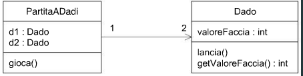
\includegraphics[scale=0.7]{images/Dadi 3.png}
\end{center}

}
\subsubsection{}
L'analisi dei requisiti e l'OOA/D vanno svolte nel contesto di un processo di sviluppo:

\begin{itemize}
    \item [$\Rightarrow$] Sviluppo iteratuivo;
    \item [$\Rightarrow$] Approccio agile;
    \item [$\Rightarrow$] Unified Process (UP).
\end{itemize}

\nt{ER e UML non sono pienamente adatti a possibili incrementi.}
\pagebreak

\subsection{UML}

\dfn{UML}{UML è un linguaggio \newfancyglitter{visuale} per la specifica,
la costruzione e la documentazione degli elaborati di un sistema software.

UML è uno standard per la notazione di diagrammi per disegnare o rappresentare
figure relative al software (specialmente OO).}
\subsubsection{}
UML è un \textit{abbozzo} o un \textit{progetto} per aiutare la comprensione nei team di sviluppo.
Il termine abbozzo indica che può essere soggetto a correzzione, ma se non ci 
sono feedback a tal proposito deve essere trattato come un dizionario.

\paragraph{Uso di UML:}

\begin{itemize}
    \item [$\Rightarrow$] Punto di vista \fancyglitter{concettuale}: modello 
    di dominio, per visualizzare concetti del mondo reale;
    \item [$\Rightarrow$] Punto di vista \fancyglitter{software}: diagramma
    delle classi di progetto, utilizzata per visualizzare elementi software.
\end{itemize}


